\section{Iteraciones del proyecto}

\subsection{Definición de los casos de uso por fase}

Los módulos que se deberían desarrollar en la fase de elaboración son
aquellos que eliminan o disminuyen los mayores riesgos del proyecto
junto con los que definen la arquitectura base del proyecto. Se decidió
que en primer fase de elaboración se desarrollaran los módulos de:

\begin{itemize}
\itemsep1pt\parskip0pt\parsep0pt
\item
  \textbf{Notificaciones y alertas}: Al tener que dar soporte no solo a
  distintos tipos de anteojos de realidad aumentada, sino también a
  otros dispositivos que nos son ahora desconocidos, creemos que este es
  uno de, sino el más, riesgoso de los módulos a implementar. El ser uno
  de los puntos fuertes de interacción con el sistema, y por lo tanto
  uno de los probables puntos de mayor \emph{carga} para el mismo,
  también es un riesgo que consideramos para tomar la decisión de elegir
  este módulo.
\item
  \textbf{Estado físico del corredor}: Consideramos que los módulos
  relacionados con la obtención y procesamiento de los datos médicos del
  corredor tienen algunos de los mayores riesgos asociados, debido a la
  heterogeneidad de datos que se podrían obtener y el desconocimiento de
  las características de procesamiento de la nube OpenStack de la
  secretaría.
\item
  \textbf{Integración con redes sociales}: El riesgo de la
  heterogeneidad de dispositivos, que también contribuye al problema de
  las notificaciones, y la falta de indicación de que redes sociales son
  las que se desea soportar nos llevan a considerar este módulo como
  riesgoso y por lo tanto a ponerlo en la primera iteración de
  elaboración. También hemos de considerar la falta de conocimiento por
  parte de los miembros del equipo del sistema Open Social.
\end{itemize}

Por lo tanto decidimos el siguiente plan de proyecto, indicado con los
casos de uso que se implementarán en cada uno, y luego incluiremos el
detalle de la primera iteración.

\begin{longtable}[c]{@{}llll@{}}
\hline\noalign{\medskip}
\begin{minipage}[b]{0.17\columnwidth}\raggedright
Fase
\end{minipage} & \begin{minipage}[b]{0.12\columnwidth}\raggedright
Número
\end{minipage} & \begin{minipage}[b]{0.58\columnwidth}\raggedright
Casos de uso
\end{minipage} & \begin{minipage}[b]{0.12\columnwidth}\raggedright
Horas
\end{minipage}
\\\noalign{\medskip}
\hline\noalign{\medskip}
\begin{minipage}[t]{0.17\columnwidth}\raggedright
Elaboración
\end{minipage} & \begin{minipage}[t]{0.12\columnwidth}\raggedright
Primera
\end{minipage} & \begin{minipage}[t]{0.58\columnwidth}\raggedright
Mostrando datos y notificaciones del entrenamiento actual.
\end{minipage} & \begin{minipage}[t]{0.12\columnwidth}\raggedright
84h
\end{minipage}
\\\noalign{\medskip}
\begin{minipage}[t]{0.17\columnwidth}\raggedright
\end{minipage} & \begin{minipage}[t]{0.12\columnwidth}\raggedright
\end{minipage} & \begin{minipage}[t]{0.58\columnwidth}\raggedright
Obteniendo posición propia y de amigos en el dispositivo empleado.
\end{minipage} & \begin{minipage}[t]{0.12\columnwidth}\raggedright
72h
\end{minipage}
\\\noalign{\medskip}
\begin{minipage}[t]{0.17\columnwidth}\raggedright
\end{minipage} & \begin{minipage}[t]{0.12\columnwidth}\raggedright
\end{minipage} & \begin{minipage}[t]{0.58\columnwidth}\raggedright
Tomando datos de estado físico del corredor.
\end{minipage} & \begin{minipage}[t]{0.12\columnwidth}\raggedright
84h
\end{minipage}
\\\noalign{\medskip}
\begin{minipage}[t]{0.17\columnwidth}\raggedright
\end{minipage} & \begin{minipage}[t]{0.12\columnwidth}\raggedright
\end{minipage} & \begin{minipage}[t]{0.58\columnwidth}\raggedright
Enviando datos a procesar a la nube local.
\end{minipage} & \begin{minipage}[t]{0.12\columnwidth}\raggedright
52h
\end{minipage}
\\\noalign{\medskip}
\begin{minipage}[t]{0.17\columnwidth}\raggedright
\end{minipage} & \begin{minipage}[t]{0.12\columnwidth}\raggedright
\end{minipage} & \begin{minipage}[t]{0.58\columnwidth}\raggedright
Compartiendo datos en tiempo real de un entrenamiento.
\end{minipage} & \begin{minipage}[t]{0.12\columnwidth}\raggedright
56h
\end{minipage}
\\\noalign{\medskip}
\begin{minipage}[t]{0.17\columnwidth}\raggedright
\end{minipage} & \begin{minipage}[t]{0.12\columnwidth}\raggedright
\end{minipage} & \begin{minipage}[t]{0.58\columnwidth}\raggedright
Logueando al usuario en el dispositivo.
\end{minipage} & \begin{minipage}[t]{0.12\columnwidth}\raggedright
112h
\end{minipage}
\\\noalign{\medskip}
\begin{minipage}[t]{0.17\columnwidth}\raggedright
Elaboración
\end{minipage} & \begin{minipage}[t]{0.12\columnwidth}\raggedright
Segunda
\end{minipage} & \begin{minipage}[t]{0.58\columnwidth}\raggedright
Levantando comentarios motivacionales de redes sociales.
\end{minipage} & \begin{minipage}[t]{0.12\columnwidth}\raggedright
60h
\end{minipage}
\\\noalign{\medskip}
\begin{minipage}[t]{0.17\columnwidth}\raggedright
\end{minipage} & \begin{minipage}[t]{0.12\columnwidth}\raggedright
\end{minipage} & \begin{minipage}[t]{0.58\columnwidth}\raggedright
Mostrando datos pedidos mediante voz.
\end{minipage} & \begin{minipage}[t]{0.12\columnwidth}\raggedright
80h
\end{minipage}
\\\noalign{\medskip}
\begin{minipage}[t]{0.17\columnwidth}\raggedright
\end{minipage} & \begin{minipage}[t]{0.12\columnwidth}\raggedright
\end{minipage} & \begin{minipage}[t]{0.58\columnwidth}\raggedright
Recibiendo notificación de necesidad de descanso.
\end{minipage} & \begin{minipage}[t]{0.12\columnwidth}\raggedright
40h
\end{minipage}
\\\noalign{\medskip}
\begin{minipage}[t]{0.17\columnwidth}\raggedright
\end{minipage} & \begin{minipage}[t]{0.12\columnwidth}\raggedright
\end{minipage} & \begin{minipage}[t]{0.58\columnwidth}\raggedright
Mostrando publicidad contextual.
\end{minipage} & \begin{minipage}[t]{0.12\columnwidth}\raggedright
120h
\end{minipage}
\\\noalign{\medskip}
\begin{minipage}[t]{0.17\columnwidth}\raggedright
Construcción
\end{minipage} & \begin{minipage}[t]{0.12\columnwidth}\raggedright
Tercera
\end{minipage} & \begin{minipage}[t]{0.58\columnwidth}\raggedright
Usando aplicación con refuerzo para discapacidad.
\end{minipage} & \begin{minipage}[t]{0.12\columnwidth}\raggedright
120h
\end{minipage}
\\\noalign{\medskip}
\begin{minipage}[t]{0.17\columnwidth}\raggedright
\end{minipage} & \begin{minipage}[t]{0.12\columnwidth}\raggedright
\end{minipage} & \begin{minipage}[t]{0.58\columnwidth}\raggedright
Iniciando un entrenamiento.
\end{minipage} & \begin{minipage}[t]{0.12\columnwidth}\raggedright
60h
\end{minipage}
\\\noalign{\medskip}
\begin{minipage}[t]{0.17\columnwidth}\raggedright
\end{minipage} & \begin{minipage}[t]{0.12\columnwidth}\raggedright
\end{minipage} & \begin{minipage}[t]{0.58\columnwidth}\raggedright
Recibiendo notificación de descanso.
\end{minipage} & \begin{minipage}[t]{0.12\columnwidth}\raggedright
80h
\end{minipage}
\\\noalign{\medskip}
\begin{minipage}[t]{0.17\columnwidth}\raggedright
\end{minipage} & \begin{minipage}[t]{0.12\columnwidth}\raggedright
\end{minipage} & \begin{minipage}[t]{0.58\columnwidth}\raggedright
Utilizando la API de datos físicos almacenados.
\end{minipage} & \begin{minipage}[t]{0.12\columnwidth}\raggedright
60h
\end{minipage}
\\\noalign{\medskip}
\begin{minipage}[t]{0.17\columnwidth}\raggedright
Construcción
\end{minipage} & \begin{minipage}[t]{0.12\columnwidth}\raggedright
Cuarta
\end{minipage} & \begin{minipage}[t]{0.58\columnwidth}\raggedright
Enviando instrucciones al corredor.
\end{minipage} & \begin{minipage}[t]{0.12\columnwidth}\raggedright
120h
\end{minipage}
\\\noalign{\medskip}
\begin{minipage}[t]{0.17\columnwidth}\raggedright
\end{minipage} & \begin{minipage}[t]{0.12\columnwidth}\raggedright
\end{minipage} & \begin{minipage}[t]{0.58\columnwidth}\raggedright
Registrando al usuario con el dispositivo.
\end{minipage} & \begin{minipage}[t]{0.12\columnwidth}\raggedright
80h
\end{minipage}
\\\noalign{\medskip}
\begin{minipage}[t]{0.17\columnwidth}\raggedright
\end{minipage} & \begin{minipage}[t]{0.12\columnwidth}\raggedright
\end{minipage} & \begin{minipage}[t]{0.58\columnwidth}\raggedright
Consumiendo comentario motivacional.
\end{minipage} & \begin{minipage}[t]{0.12\columnwidth}\raggedright
60h
\end{minipage}
\\\noalign{\medskip}
\begin{minipage}[t]{0.17\columnwidth}\raggedright
\end{minipage} & \begin{minipage}[t]{0.12\columnwidth}\raggedright
\end{minipage} & \begin{minipage}[t]{0.58\columnwidth}\raggedright
Corriendo carrera virtual.
\end{minipage} & \begin{minipage}[t]{0.12\columnwidth}\raggedright
40h
\end{minipage}
\\\noalign{\medskip}
\begin{minipage}[t]{0.17\columnwidth}\raggedright
\end{minipage} & \begin{minipage}[t]{0.12\columnwidth}\raggedright
\end{minipage} & \begin{minipage}[t]{0.58\columnwidth}\raggedright
Añadiendo publicidad al sistema.
\end{minipage} & \begin{minipage}[t]{0.12\columnwidth}\raggedright
120h
\end{minipage}
\\\noalign{\medskip}
\begin{minipage}[t]{0.17\columnwidth}\raggedright
Construcción
\end{minipage} & \begin{minipage}[t]{0.12\columnwidth}\raggedright
Quinta
\end{minipage} & \begin{minipage}[t]{0.58\columnwidth}\raggedright
Enviando instrucciones al corredor.
\end{minipage} & \begin{minipage}[t]{0.12\columnwidth}\raggedright
80h
\end{minipage}
\\\noalign{\medskip}
\begin{minipage}[t]{0.17\columnwidth}\raggedright
\end{minipage} & \begin{minipage}[t]{0.12\columnwidth}\raggedright
\end{minipage} & \begin{minipage}[t]{0.58\columnwidth}\raggedright
Consumiendo instrucciones del entrenador.
\end{minipage} & \begin{minipage}[t]{0.12\columnwidth}\raggedright
80h
\end{minipage}
\\\noalign{\medskip}
\begin{minipage}[t]{0.17\columnwidth}\raggedright
\end{minipage} & \begin{minipage}[t]{0.12\columnwidth}\raggedright
\end{minipage} & \begin{minipage}[t]{0.58\columnwidth}\raggedright
Mostrando publicidad en carrera.
\end{minipage} & \begin{minipage}[t]{0.12\columnwidth}\raggedright
120h
\end{minipage}
\\\noalign{\medskip}
\begin{minipage}[t]{0.17\columnwidth}\raggedright
\end{minipage} & \begin{minipage}[t]{0.12\columnwidth}\raggedright
\end{minipage} & \begin{minipage}[t]{0.58\columnwidth}\raggedright
Iniciando un entrenamiento.
\end{minipage} & \begin{minipage}[t]{0.12\columnwidth}\raggedright
60h
\end{minipage}
\\\noalign{\medskip}
\hline
\end{longtable}

Con lo cual tenemos un total de 480 horas, que considerando la
conformación de equipo dada anteriormente, corresponde a la cantidad de
horas hombre disponibles.

\subsection{Detalle de tareas para la primera iteración}

\subsubsection{Casos de uso y tareas}

A continuación incluimos las tareas a realizar con sus dependencias,
para la primer iteración (correspondiente a la primera fase de
elaboración presentada anteriormente).

\begin{longtable}[c]{@{}lll@{}}
\hline\noalign{\medskip}
\begin{minipage}[b]{0.28\columnwidth}\raggedright
Caso de uso
\end{minipage} & \begin{minipage}[b]{0.62\columnwidth}\raggedright
Tarea
\end{minipage} & \begin{minipage}[b]{0.10\columnwidth}\raggedright
Horas
\end{minipage}
\\\noalign{\medskip}
\hline\noalign{\medskip}
\begin{minipage}[t]{0.28\columnwidth}\raggedright
Logueando al usuario en el dispositivo
\end{minipage} & \begin{minipage}[t]{0.62\columnwidth}\raggedright
Investigar la arquitectura de login en Open Social.
\end{minipage} & \begin{minipage}[t]{0.10\columnwidth}\raggedright
8h
\end{minipage}
\\\noalign{\medskip}
\begin{minipage}[t]{0.28\columnwidth}\raggedright
\end{minipage} & \begin{minipage}[t]{0.62\columnwidth}\raggedright
Validar con los \emph{stakeholders} que tipo de sistemas de entrada
deben soportar los dispositivos.
\end{minipage} & \begin{minipage}[t]{0.10\columnwidth}\raggedright
4h
\end{minipage}
\\\noalign{\medskip}
\begin{minipage}[t]{0.28\columnwidth}\raggedright
\end{minipage} & \begin{minipage}[t]{0.62\columnwidth}\raggedright
Implementar capa de abstracción para interactuar con los dispositivos a
soportar y determinar sus características.
\end{minipage} & \begin{minipage}[t]{0.10\columnwidth}\raggedright
16h
\end{minipage}
\\\noalign{\medskip}
\begin{minipage}[t]{0.28\columnwidth}\raggedright
\end{minipage} & \begin{minipage}[t]{0.62\columnwidth}\raggedright
Implementar sistema de \emph{login} para cada dispositivo a soportar.
\end{minipage} & \begin{minipage}[t]{0.10\columnwidth}\raggedright
16h
\end{minipage}
\\\noalign{\medskip}
\begin{minipage}[t]{0.28\columnwidth}\raggedright
\end{minipage} & \begin{minipage}[t]{0.62\columnwidth}\raggedright
Diseñar e implementar mecanismos de logueo externos para soportar
dispositivos sin interfaz de entrada.
\end{minipage} & \begin{minipage}[t]{0.10\columnwidth}\raggedright
28h
\end{minipage}
\\\noalign{\medskip}
\begin{minipage}[t]{0.28\columnwidth}\raggedright
\end{minipage} & \begin{minipage}[t]{0.62\columnwidth}\raggedright
Implementar capa de interacción con redes sociales a soportar para
permitir el registro.
\end{minipage} & \begin{minipage}[t]{0.10\columnwidth}\raggedright
16h
\end{minipage}
\\\noalign{\medskip}
\begin{minipage}[t]{0.28\columnwidth}\raggedright
\end{minipage} & \begin{minipage}[t]{0.62\columnwidth}\raggedright
Diseñar módulos de interfaz con el dispositivo.
\end{minipage} & \begin{minipage}[t]{0.10\columnwidth}\raggedright
8h
\end{minipage}
\\\noalign{\medskip}
\begin{minipage}[t]{0.28\columnwidth}\raggedright
\end{minipage} & \begin{minipage}[t]{0.62\columnwidth}\raggedright
Documentar las interfaces esperadas de los dispositivos.
\end{minipage} & \begin{minipage}[t]{0.10\columnwidth}\raggedright
4h
\end{minipage}
\\\noalign{\medskip}
\begin{minipage}[t]{0.28\columnwidth}\raggedright
\end{minipage} & \begin{minipage}[t]{0.62\columnwidth}\raggedright
Testeo y \emph{debugging} de las implementaciones particulares y de la
interfaz general
\end{minipage} & \begin{minipage}[t]{0.10\columnwidth}\raggedright
4h
\end{minipage}
\\\noalign{\medskip}
\begin{minipage}[t]{0.28\columnwidth}\raggedright
\end{minipage} & \begin{minipage}[t]{0.62\columnwidth}\raggedright
Separar los tipos de usuarios entre corredores, entrenadores y
comentadores.
\end{minipage} & \begin{minipage}[t]{0.10\columnwidth}\raggedright
4h
\end{minipage}
\\\noalign{\medskip}
\begin{minipage}[t]{0.28\columnwidth}\raggedright
Mostrando datos y notificaciones
\end{minipage} & \begin{minipage}[t]{0.62\columnwidth}\raggedright
Validar con los \emph{stakeholders} que tipos de sistemas de aviso de
información han de soportar los dispositivos.
\end{minipage} & \begin{minipage}[t]{0.10\columnwidth}\raggedright
4h
\end{minipage}
\\\noalign{\medskip}
\begin{minipage}[t]{0.28\columnwidth}\raggedright
\end{minipage} & \begin{minipage}[t]{0.62\columnwidth}\raggedright
Implementar una capa de detección y abstracción de características de
notificación al usuario para los dispositivos.
\end{minipage} & \begin{minipage}[t]{0.10\columnwidth}\raggedright
30h
\end{minipage}
\\\noalign{\medskip}
\begin{minipage}[t]{0.28\columnwidth}\raggedright
\end{minipage} & \begin{minipage}[t]{0.62\columnwidth}\raggedright
Determinar que tipo de datos notificar al usuario sin que este los
demande.
\end{minipage} & \begin{minipage}[t]{0.10\columnwidth}\raggedright
4h
\end{minipage}
\\\noalign{\medskip}
\begin{minipage}[t]{0.28\columnwidth}\raggedright
\end{minipage} & \begin{minipage}[t]{0.62\columnwidth}\raggedright
Implementar una interfaz para soportar distintos tipos de datos a
notificar.
\end{minipage} & \begin{minipage}[t]{0.10\columnwidth}\raggedright
8h
\end{minipage}
\\\noalign{\medskip}
\begin{minipage}[t]{0.28\columnwidth}\raggedright
\end{minipage} & \begin{minipage}[t]{0.62\columnwidth}\raggedright
Implementar para cada dispositivo la metodología de envio de
notificaciones que se ajuste a sus capacidades técnicas.
\end{minipage} & \begin{minipage}[t]{0.10\columnwidth}\raggedright
30h
\end{minipage}
\\\noalign{\medskip}
\begin{minipage}[t]{0.28\columnwidth}\raggedright
\end{minipage} & \begin{minipage}[t]{0.62\columnwidth}\raggedright
Documentar las interfaces esperadas de los dispositivos.
\end{minipage} & \begin{minipage}[t]{0.10\columnwidth}\raggedright
4h
\end{minipage}
\\\noalign{\medskip}
\begin{minipage}[t]{0.28\columnwidth}\raggedright
\end{minipage} & \begin{minipage}[t]{0.62\columnwidth}\raggedright
Testeo y \emph{debugging} de las implementaciones particulares y de la
interfaz general.
\end{minipage} & \begin{minipage}[t]{0.10\columnwidth}\raggedright
4h
\end{minipage}
\\\noalign{\medskip}
\begin{minipage}[t]{0.28\columnwidth}\raggedright
Compartiendo datos en tiempo real de un entrenamiento
\end{minipage} & \begin{minipage}[t]{0.62\columnwidth}\raggedright
Investigar como compartir datos bajo Open Social
\end{minipage} & \begin{minipage}[t]{0.10\columnwidth}\raggedright
8h
\end{minipage}
\\\noalign{\medskip}
\begin{minipage}[t]{0.28\columnwidth}\raggedright
\end{minipage} & \begin{minipage}[t]{0.62\columnwidth}\raggedright
Implementar sistema de \emph{social sharing} para cada red social a dar
soporte en esta instancia.
\end{minipage} & \begin{minipage}[t]{0.10\columnwidth}\raggedright
16h
\end{minipage}
\\\noalign{\medskip}
\begin{minipage}[t]{0.28\columnwidth}\raggedright
\end{minipage} & \begin{minipage}[t]{0.62\columnwidth}\raggedright
Integrar sistema de \emph{login} a este módulo.
\end{minipage} & \begin{minipage}[t]{0.10\columnwidth}\raggedright
8h
\end{minipage}
\\\noalign{\medskip}
\begin{minipage}[t]{0.28\columnwidth}\raggedright
\end{minipage} & \begin{minipage}[t]{0.62\columnwidth}\raggedright
Validar políticas de privacidad de datos con \emph{stakeholders}
\end{minipage} & \begin{minipage}[t]{0.10\columnwidth}\raggedright
4h
\end{minipage}
\\\noalign{\medskip}
\begin{minipage}[t]{0.28\columnwidth}\raggedright
\end{minipage} & \begin{minipage}[t]{0.62\columnwidth}\raggedright
Testeo y \emph{debugging} del módulo.
\end{minipage} & \begin{minipage}[t]{0.10\columnwidth}\raggedright
4h
\end{minipage}
\\\noalign{\medskip}
\begin{minipage}[t]{0.28\columnwidth}\raggedright
Obteniendo posición propia y de amigos en el dispositivo empleado.
\end{minipage} & \begin{minipage}[t]{0.62\columnwidth}\raggedright
Validar con los \emph{stakeholders} que tipo de geolocalización se se
desea soportar.
\end{minipage} & \begin{minipage}[t]{0.10\columnwidth}\raggedright
4h
\end{minipage}
\\\noalign{\medskip}
\begin{minipage}[t]{0.28\columnwidth}\raggedright
\end{minipage} & \begin{minipage}[t]{0.62\columnwidth}\raggedright
Implementación de obtención de datos de geolocalización.
\end{minipage} & \begin{minipage}[t]{0.10\columnwidth}\raggedright
24h
\end{minipage}
\\\noalign{\medskip}
\begin{minipage}[t]{0.28\columnwidth}\raggedright
\end{minipage} & \begin{minipage}[t]{0.62\columnwidth}\raggedright
Implementación de sistema de notificación de geolocalización.
\end{minipage} & \begin{minipage}[t]{0.10\columnwidth}\raggedright
24h
\end{minipage}
\\\noalign{\medskip}
\begin{minipage}[t]{0.28\columnwidth}\raggedright
\end{minipage} & \begin{minipage}[t]{0.62\columnwidth}\raggedright
Integración con el módulo de \emph{social sharing}.
\end{minipage} & \begin{minipage}[t]{0.10\columnwidth}\raggedright
8h
\end{minipage}
\\\noalign{\medskip}
\begin{minipage}[t]{0.28\columnwidth}\raggedright
\end{minipage} & \begin{minipage}[t]{0.62\columnwidth}\raggedright
Testeo y \emph{debugging} del módulo.
\end{minipage} & \begin{minipage}[t]{0.10\columnwidth}\raggedright
4h
\end{minipage}
\\\noalign{\medskip}
\begin{minipage}[t]{0.28\columnwidth}\raggedright
Tomando datos de estado físico del corredor.
\end{minipage} & \begin{minipage}[t]{0.62\columnwidth}\raggedright
Validar que tipos de dispositivos médicos se van a soportar.
\end{minipage} & \begin{minipage}[t]{0.10\columnwidth}\raggedright
4h
\end{minipage}
\\\noalign{\medskip}
\begin{minipage}[t]{0.28\columnwidth}\raggedright
\end{minipage} & \begin{minipage}[t]{0.62\columnwidth}\raggedright
Implementar el módulo de detección de capacidades de medición para datos
biomédicos
\end{minipage} & \begin{minipage}[t]{0.10\columnwidth}\raggedright
32h
\end{minipage}
\\\noalign{\medskip}
\begin{minipage}[t]{0.28\columnwidth}\raggedright
\end{minipage} & \begin{minipage}[t]{0.62\columnwidth}\raggedright
Implementar módulo de medición para los dispositivos médicos.
\end{minipage} & \begin{minipage}[t]{0.10\columnwidth}\raggedright
32h
\end{minipage}
\\\noalign{\medskip}
\begin{minipage}[t]{0.28\columnwidth}\raggedright
\end{minipage} & \begin{minipage}[t]{0.62\columnwidth}\raggedright
Documentación de las interfaces esperadas.
\end{minipage} & \begin{minipage}[t]{0.10\columnwidth}\raggedright
4h
\end{minipage}
\\\noalign{\medskip}
\begin{minipage}[t]{0.28\columnwidth}\raggedright
\end{minipage} & \begin{minipage}[t]{0.62\columnwidth}\raggedright
Testeo y \emph{debugging} de la implementación.
\end{minipage} & \begin{minipage}[t]{0.10\columnwidth}\raggedright
8h
\end{minipage}
\\\noalign{\medskip}
\begin{minipage}[t]{0.28\columnwidth}\raggedright
Enviando datos a procesar a la nube local.
\end{minipage} & \begin{minipage}[t]{0.62\columnwidth}\raggedright
Investigar la plataforma Open Stack.
\end{minipage} & \begin{minipage}[t]{0.10\columnwidth}\raggedright
4h
\end{minipage}
\\\noalign{\medskip}
\begin{minipage}[t]{0.28\columnwidth}\raggedright
\end{minipage} & \begin{minipage}[t]{0.62\columnwidth}\raggedright
Implementar adaptador para llegada de datos a la nube de Secretaría.
\end{minipage} & \begin{minipage}[t]{0.10\columnwidth}\raggedright
8h
\end{minipage}
\\\noalign{\medskip}
\begin{minipage}[t]{0.28\columnwidth}\raggedright
\end{minipage} & \begin{minipage}[t]{0.62\columnwidth}\raggedright
Conseguir especificación técnica del software de procesamiento de datos
de la Secretaría.
\end{minipage} & \begin{minipage}[t]{0.10\columnwidth}\raggedright
16h
\end{minipage}
\\\noalign{\medskip}
\begin{minipage}[t]{0.28\columnwidth}\raggedright
\end{minipage} & \begin{minipage}[t]{0.62\columnwidth}\raggedright
Implementar módulo de envío de datos a la Secretaría.
\end{minipage} & \begin{minipage}[t]{0.10\columnwidth}\raggedright
8h
\end{minipage}
\\\noalign{\medskip}
\begin{minipage}[t]{0.28\columnwidth}\raggedright
\end{minipage} & \begin{minipage}[t]{0.62\columnwidth}\raggedright
Documentar la interfaz con el sistema.
\end{minipage} & \begin{minipage}[t]{0.10\columnwidth}\raggedright
8h
\end{minipage}
\\\noalign{\medskip}
\begin{minipage}[t]{0.28\columnwidth}\raggedright
\end{minipage} & \begin{minipage}[t]{0.62\columnwidth}\raggedright
Testeo y \emph{debugging} de la implementación.
\end{minipage} & \begin{minipage}[t]{0.10\columnwidth}\raggedright
4h
\end{minipage}
\\\noalign{\medskip}
\hline
\end{longtable}

En total tenemos entonces 460 horas, lo que nos da un poco de
\textbf{slack} en la iteración considerando la posibilidad de que surga
un evento inesperado o nuestras estimaciones sean incorrectas.

% \subsubsection{Diagrama GANTT de la iteración}
% Incuimos a continuación el diagrama de \texttt{GANTT} detallado:

\begin{figure}[c]
  \label{diag_diseno}
  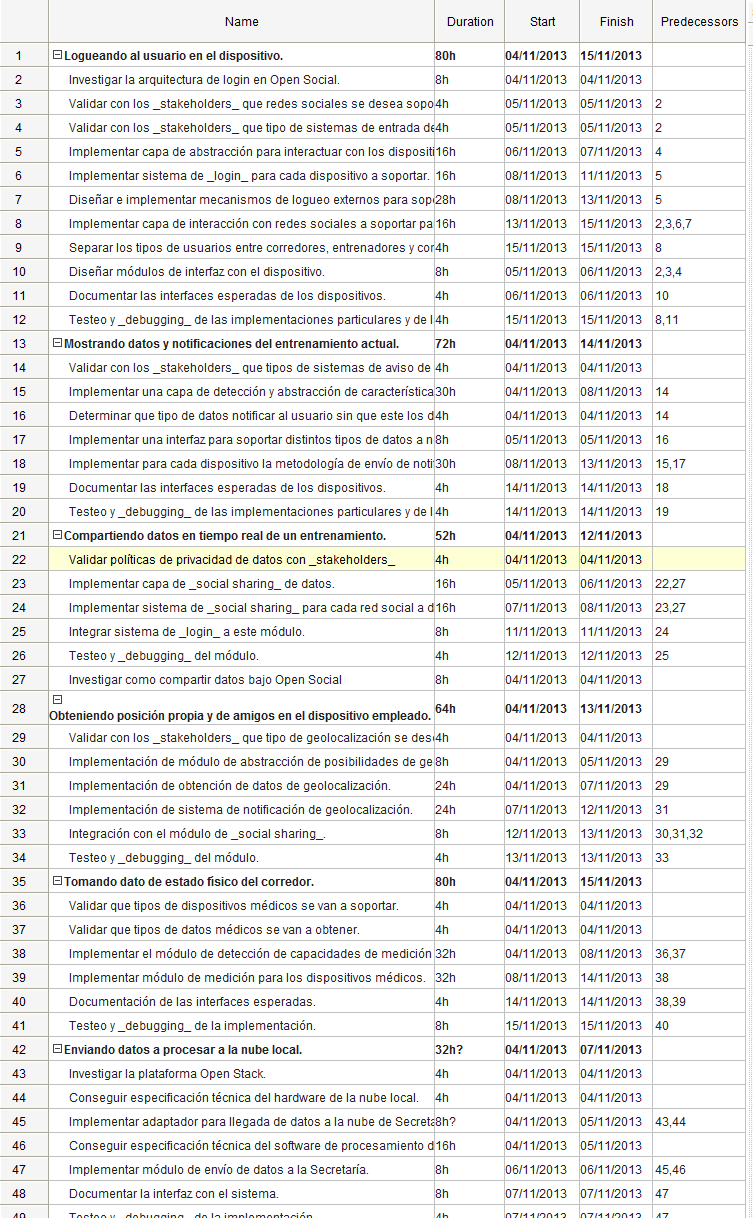
\includegraphics[scale=0.75]{images/GANTTABLE.png}
  \caption{Diagrama de \texttt{GANTT}}
\end{figure} 

\begin{landscape}
\begin{figure}[c]
  \label{diag_diseno}
  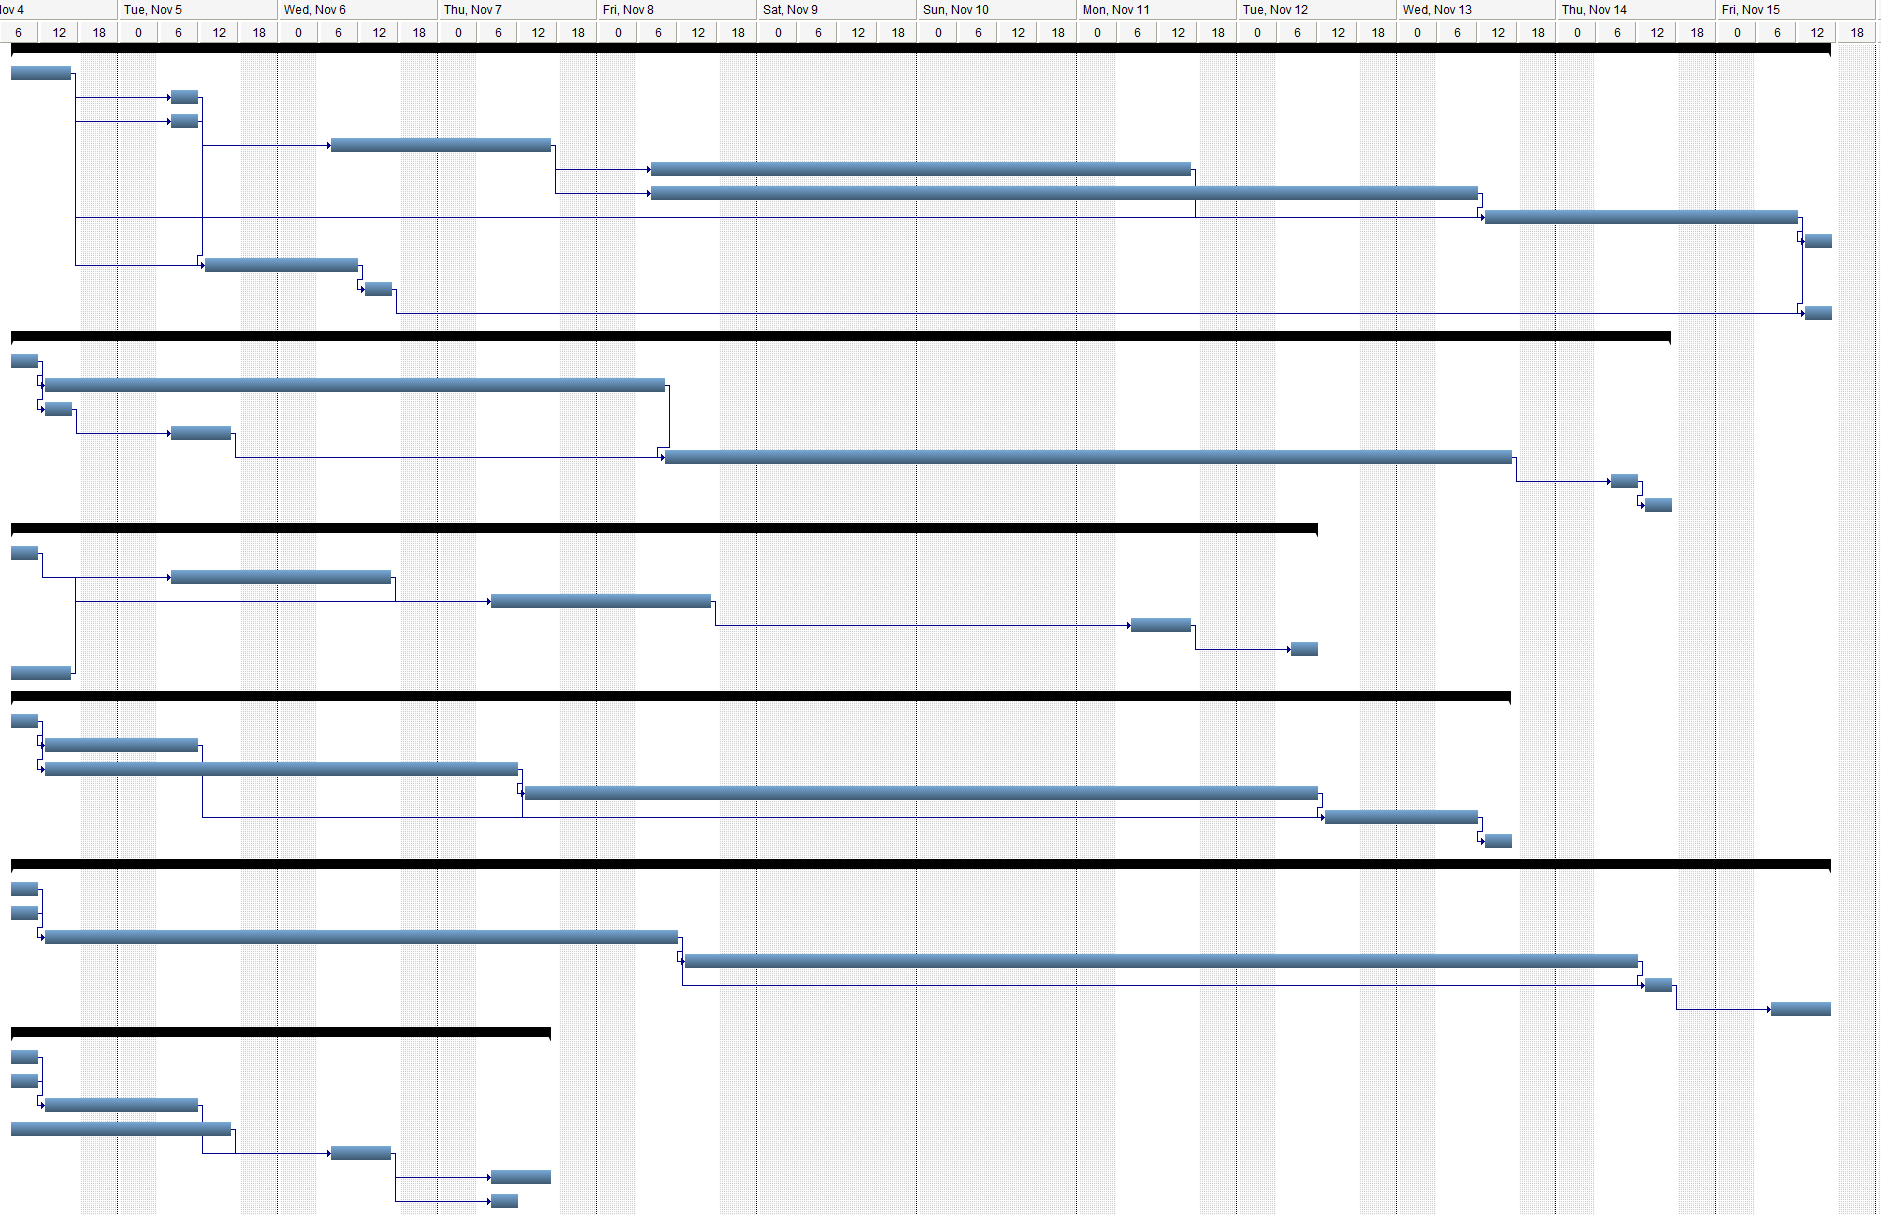
\includegraphics[scale=0.5]{images/GANTGRAPH.png}
  \caption{Diagrama de \texttt{GANTT}}
\end{figure} 
\end{landscape}
